\documentclass[]{article}
\usepackage[T1]{fontenc}
\usepackage{lmodern}
\usepackage{amssymb,amsmath}
\usepackage{ifxetex,ifluatex}
\usepackage{fixltx2e} % provides \textsubscript
% Set line spacing
% use upquote if available, for straight quotes in verbatim environments
\IfFileExists{upquote.sty}{\usepackage{upquote}}{}
\ifnum 0\ifxetex 1\fi\ifluatex 1\fi=0 % if pdftex
  \usepackage[utf8]{inputenc}
\else % if luatex or xelatex
  \ifxetex
    \usepackage{mathspec}
    \usepackage{xltxtra,xunicode}
  \else
    \usepackage{fontspec}
  \fi
  \defaultfontfeatures{Mapping=tex-text,Scale=MatchLowercase}
  \newcommand{\euro}{€}
\fi
% use microtype if available
\IfFileExists{microtype.sty}{\usepackage{microtype}}{}
\usepackage[margin=1in]{geometry}
\usepackage{color}
\usepackage{fancyvrb}
\newcommand{\VerbBar}{|}
\newcommand{\VERB}{\Verb[commandchars=\\\{\}]}
\DefineVerbatimEnvironment{Highlighting}{Verbatim}{commandchars=\\\{\}}
% Add ',fontsize=\small' for more characters per line
\usepackage{framed}
\definecolor{shadecolor}{RGB}{248,248,248}
\newenvironment{Shaded}{\begin{snugshade}}{\end{snugshade}}
\newcommand{\KeywordTok}[1]{\textcolor[rgb]{0.13,0.29,0.53}{\textbf{{#1}}}}
\newcommand{\DataTypeTok}[1]{\textcolor[rgb]{0.13,0.29,0.53}{{#1}}}
\newcommand{\DecValTok}[1]{\textcolor[rgb]{0.00,0.00,0.81}{{#1}}}
\newcommand{\BaseNTok}[1]{\textcolor[rgb]{0.00,0.00,0.81}{{#1}}}
\newcommand{\FloatTok}[1]{\textcolor[rgb]{0.00,0.00,0.81}{{#1}}}
\newcommand{\CharTok}[1]{\textcolor[rgb]{0.31,0.60,0.02}{{#1}}}
\newcommand{\StringTok}[1]{\textcolor[rgb]{0.31,0.60,0.02}{{#1}}}
\newcommand{\CommentTok}[1]{\textcolor[rgb]{0.56,0.35,0.01}{\textit{{#1}}}}
\newcommand{\OtherTok}[1]{\textcolor[rgb]{0.56,0.35,0.01}{{#1}}}
\newcommand{\AlertTok}[1]{\textcolor[rgb]{0.94,0.16,0.16}{{#1}}}
\newcommand{\FunctionTok}[1]{\textcolor[rgb]{0.00,0.00,0.00}{{#1}}}
\newcommand{\RegionMarkerTok}[1]{{#1}}
\newcommand{\ErrorTok}[1]{\textbf{{#1}}}
\newcommand{\NormalTok}[1]{{#1}}
\usepackage{graphicx}
% Redefine \includegraphics so that, unless explicit options are
% given, the image width will not exceed the width of the page.
% Images get their normal width if they fit onto the page, but
% are scaled down if they would overflow the margins.
\makeatletter
\def\ScaleIfNeeded{%
  \ifdim\Gin@nat@width>\linewidth
    \linewidth
  \else
    \Gin@nat@width
  \fi
}
\makeatother
\let\Oldincludegraphics\includegraphics
{%
 \catcode`\@=11\relax%
 \gdef\includegraphics{\@ifnextchar[{\Oldincludegraphics}{\Oldincludegraphics[width=\ScaleIfNeeded]}}%
}%
\ifxetex
  \usepackage[setpagesize=false, % page size defined by xetex
              unicode=false, % unicode breaks when used with xetex
              xetex]{hyperref}
\else
  \usepackage[unicode=true]{hyperref}
\fi
\hypersetup{breaklinks=true,
            bookmarks=true,
            pdfauthor={},
            pdftitle={Practical Machine Learning Assignment},
            colorlinks=true,
            citecolor=blue,
            urlcolor=blue,
            linkcolor=magenta,
            pdfborder={0 0 0}}
\urlstyle{same}  % don't use monospace font for urls
\setlength{\parindent}{0pt}
\setlength{\parskip}{6pt plus 2pt minus 1pt}
\setlength{\emergencystretch}{3em}  % prevent overfull lines
\setcounter{secnumdepth}{0}

%%% Change title format to be more compact
\usepackage{titling}
\setlength{\droptitle}{-2em}
  \title{Practical Machine Learning Assignment}
  \pretitle{\vspace{\droptitle}\centering\huge}
  \posttitle{\par}
  \author{}
  \preauthor{}\postauthor{}
  \date{}
  \predate{}\postdate{}




\begin{document}

\maketitle


\subsection{Executive summary}\label{executive-summary}

Analyze the device data from Jawbone Up, Nike FuelBand, and Fitbit for 6
participants, from their accelerometers on the belt, forearm, arm, and
dumbelldata for 5 dataset using linear regression models. This learning
will quantify how much of a particular activity they do, but they rarely
quantify how well they do it.

\subsection{Reading the data}\label{reading-the-data}

\subsubsection{The Raw Data - Download the file if does not exist in
local
system}\label{the-raw-data---download-the-file-if-does-not-exist-in-local-system}

\begin{Shaded}
\begin{Highlighting}[]
\NormalTok{if (!}\KeywordTok{file.exists}\NormalTok{(}\StringTok{"./Data/pml-training.csv"}\NormalTok{))\{}
  \KeywordTok{download.file}\NormalTok{(}\StringTok{"https://d396qusza40orc.cloudfront.net/predmachlearn/pml-training.csv"}\NormalTok{,}
                \StringTok{"./Data/pml-training.csv"}\NormalTok{)}
\NormalTok{\}}
\NormalTok{if (!}\KeywordTok{file.exists}\NormalTok{(}\StringTok{"./Data/pml-testing.csv"}\NormalTok{))\{}
  \KeywordTok{download.file}\NormalTok{(}\StringTok{"https://d396qusza40orc.cloudfront.net/predmachlearn/pml-training.csv"}\NormalTok{,}
                \StringTok{"./Data/pml-testing.csv"}\NormalTok{)}
\NormalTok{\}}
\end{Highlighting}
\end{Shaded}

\subsubsection{Load the training and testing
data}\label{load-the-training-and-testing-data}

\begin{Shaded}
\begin{Highlighting}[]
\NormalTok{trainingdata =}\StringTok{ }\KeywordTok{read.csv}\NormalTok{(}\StringTok{"./Data/pml-training.csv"}\NormalTok{, }\DataTypeTok{na.strings =} \KeywordTok{c}\NormalTok{(}\StringTok{"NA"}\NormalTok{, }\StringTok{""}\NormalTok{))}
\KeywordTok{dim}\NormalTok{(trainingdata); }\KeywordTok{summary}\NormalTok{(trainingdata$classe)}
\end{Highlighting}
\end{Shaded}

\begin{verbatim}
## [1] 19622   160
\end{verbatim}

\begin{verbatim}
##    A    B    C    D    E 
## 5580 3797 3422 3216 3607
\end{verbatim}

\begin{Shaded}
\begin{Highlighting}[]
\NormalTok{testingdata =}\StringTok{ }\KeywordTok{read.csv}\NormalTok{(}\StringTok{"./Data/pml-testing.csv"}\NormalTok{, }\DataTypeTok{na.strings =} \KeywordTok{c}\NormalTok{(}\StringTok{"NA"}\NormalTok{, }\StringTok{""}\NormalTok{))}
\end{Highlighting}
\end{Shaded}

\subsubsection{Load the library}\label{load-the-library}

\begin{Shaded}
\begin{Highlighting}[]
\KeywordTok{library}\NormalTok{(ggplot2); }\KeywordTok{library}\NormalTok{(caret);}\KeywordTok{library}\NormalTok{(randomForest)}
\end{Highlighting}
\end{Shaded}

\subsubsection{Removing near Zero
covariates}\label{removing-near-zero-covariates}

\begin{Shaded}
\begin{Highlighting}[]
\NormalTok{nzv <-}\StringTok{ }\KeywordTok{nearZeroVar}\NormalTok{(trainingdata,}\DataTypeTok{saveMetrics=}\OtherTok{TRUE}\NormalTok{)}
\NormalTok{trainingdata <-}\StringTok{ }\NormalTok{trainingdata[,nzv$nzv==}\OtherTok{FALSE}\NormalTok{]}

\NormalTok{nzv <-}\StringTok{ }\KeywordTok{nearZeroVar}\NormalTok{(testingdata,}\DataTypeTok{saveMetrics=}\OtherTok{TRUE}\NormalTok{)}
\NormalTok{testingdata <-}\StringTok{ }\NormalTok{testingdata[,nzv$nzv==}\OtherTok{FALSE}\NormalTok{]}
\end{Highlighting}
\end{Shaded}

\subsection{Partioning the training
datset}\label{partioning-the-training-datset}

\begin{Shaded}
\begin{Highlighting}[]
\NormalTok{inTrain <-}\StringTok{ }\KeywordTok{createDataPartition}\NormalTok{(}\DataTypeTok{y=}\NormalTok{trainingdata$classe, }\DataTypeTok{p=}\FloatTok{0.6}\NormalTok{, }\DataTypeTok{list=}\OtherTok{FALSE}\NormalTok{)}
\NormalTok{projTraining <-}\StringTok{ }\NormalTok{trainingdata[inTrain, ]; projTesting <-}\StringTok{ }\NormalTok{trainingdata[-inTrain, ]}
\KeywordTok{dim}\NormalTok{(projTraining); }\KeywordTok{dim}\NormalTok{(projTesting)}
\end{Highlighting}
\end{Shaded}

\begin{verbatim}
## [1] 11776   117
\end{verbatim}

\begin{verbatim}
## [1] 7846  117
\end{verbatim}

\subsubsection{Killing first column of Dataset(ID Removing first ID
variable) so that it does not interfer with ML
Algorithms.}\label{killing-first-column-of-datasetid-removing-first-id-variable-so-that-it-does-not-interfer-with-ml-algorithms.}

\begin{Shaded}
\begin{Highlighting}[]
\NormalTok{projTraining <-}\StringTok{ }\NormalTok{projTraining[}\KeywordTok{c}\NormalTok{(-}\DecValTok{1}\NormalTok{)]}
\end{Highlighting}
\end{Shaded}

\subsubsection{Remove the columns / Variables has too many NAs (keep
only the variable \textgreater{} 60\% threshold of
NA's)}\label{remove-the-columns-variables-has-too-many-nas-keep-only-the-variable-60-threshold-of-nas}

\begin{Shaded}
\begin{Highlighting}[]
\NormalTok{subprojTraining <-}\StringTok{ }\NormalTok{projTraining }
\NormalTok{for(i in }\DecValTok{1}\NormalTok{:}\KeywordTok{length}\NormalTok{(projTraining)) \{ }
  \NormalTok{if( }\KeywordTok{sum}\NormalTok{( }\KeywordTok{is.na}\NormalTok{( projTraining[, i] ) ) /}\KeywordTok{nrow}\NormalTok{(projTraining) >=}\StringTok{ }\NormalTok{.}\DecValTok{6} \NormalTok{) \{ }
    \NormalTok{for(j in }\DecValTok{1}\NormalTok{:}\KeywordTok{length}\NormalTok{(subprojTraining)) \{}
      \NormalTok{if( }\KeywordTok{length}\NormalTok{( }\KeywordTok{grep}\NormalTok{(}\KeywordTok{names}\NormalTok{(projTraining[i]), }\KeywordTok{names}\NormalTok{(subprojTraining)[j]) ) ==}\DecValTok{1}\NormalTok{)  \{ }
        \NormalTok{subprojTraining <-}\StringTok{ }\NormalTok{subprojTraining[ , -j] }
      \NormalTok{\}   }
    \NormalTok{\} }
  \NormalTok{\}}
\NormalTok{\}}

\NormalTok{projTraining <-}\StringTok{ }\NormalTok{subprojTraining}
\KeywordTok{rm}\NormalTok{(subprojTraining)}

\NormalTok{clean1 <-}\StringTok{ }\KeywordTok{colnames}\NormalTok{(projTraining)}
\NormalTok{clean2 <-}\StringTok{ }\KeywordTok{colnames}\NormalTok{(projTraining[, -}\DecValTok{58}\NormalTok{]) }\CommentTok{# Remove the classe column }
\NormalTok{projTesting <-}\StringTok{ }\NormalTok{projTesting[clean1]; }\CommentTok{# set/allow same variabels which are in Training}
\NormalTok{testing <-}\StringTok{ }\NormalTok{testingdata[clean2] }\CommentTok{# allow same variables which are in training}

\KeywordTok{dim}\NormalTok{(projTesting); }\KeywordTok{dim}\NormalTok{(testing)}
\end{Highlighting}
\end{Shaded}

\begin{verbatim}
## [1] 7846   58
\end{verbatim}

\begin{verbatim}
## [1] 20 57
\end{verbatim}

\subsection{Coerce the data into the same
type}\label{coerce-the-data-into-the-same-type}

\begin{Shaded}
\begin{Highlighting}[]
\NormalTok{for (i in }\DecValTok{1}\NormalTok{:}\KeywordTok{length}\NormalTok{(testing) ) \{}
    \NormalTok{for(j in }\DecValTok{1}\NormalTok{:}\KeywordTok{length}\NormalTok{(projTraining)) \{}
        \NormalTok{if( }\KeywordTok{length}\NormalTok{( }\KeywordTok{grep}\NormalTok{(}\KeywordTok{names}\NormalTok{(projTraining[i]), }\KeywordTok{names}\NormalTok{(testing)[j]) ) ==}\StringTok{ }\DecValTok{1}\NormalTok{)  \{}
            \KeywordTok{class}\NormalTok{(testing[j]) <-}\StringTok{ }\KeywordTok{class}\NormalTok{(projTraining[i])}
        \NormalTok{\}      }
    \NormalTok{\}      }
\NormalTok{\}}

\CommentTok{# To get the same class between testing and myTraining}
\NormalTok{testing <-}\StringTok{ }\KeywordTok{rbind}\NormalTok{(projTraining[}\DecValTok{2}\NormalTok{, -}\DecValTok{58}\NormalTok{] , testing)}
\NormalTok{testing <-}\StringTok{ }\NormalTok{testing[-}\DecValTok{1}\NormalTok{,]}
\end{Highlighting}
\end{Shaded}

\subsection{Model Builinding \textasciitilde{} Train model with random
forest due to its highly accuracy
rate.}\label{model-builinding-train-model-with-random-forest-due-to-its-highly-accuracy-rate.}

\begin{Shaded}
\begin{Highlighting}[]
\KeywordTok{set.seed}\NormalTok{(}\DecValTok{12345}\NormalTok{)}
\NormalTok{modFit1 <-}\StringTok{ }\KeywordTok{randomForest}\NormalTok{(classe ~. , }\DataTypeTok{data=}\NormalTok{projTraining)}
\KeywordTok{plot}\NormalTok{(modFit1)}
\end{Highlighting}
\end{Shaded}

\begin{figure}[htbp]
\centering
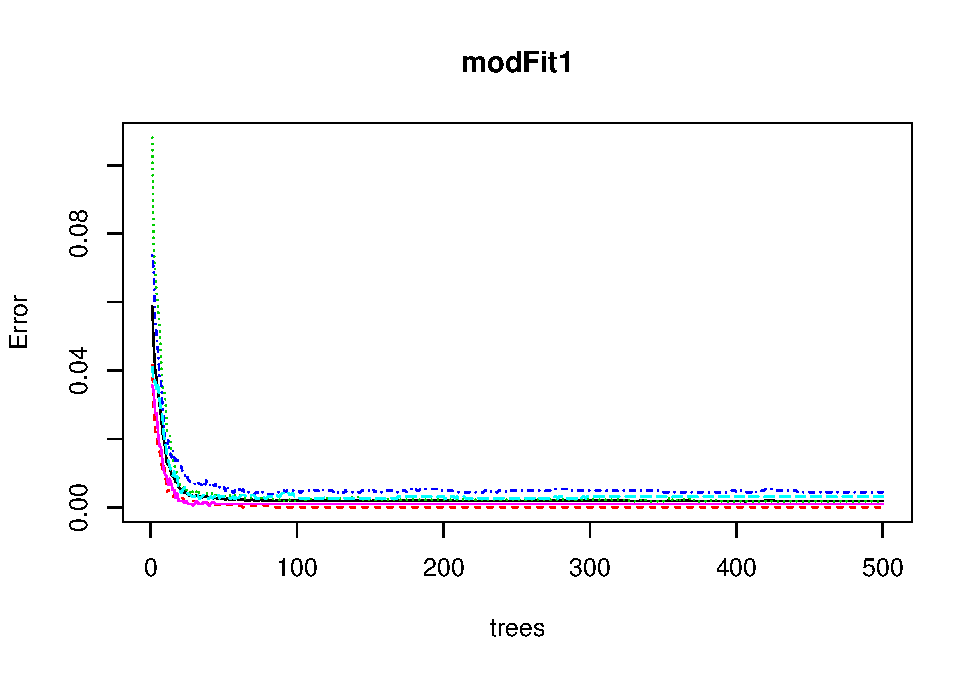
\includegraphics{ML_Project_files/figure-latex/unnamed-chunk-9-1.pdf}
\caption{}
\end{figure}

\begin{Shaded}
\begin{Highlighting}[]
\NormalTok{predict1 <-}\StringTok{ }\KeywordTok{predict}\NormalTok{(modFit1, projTesting, }\DataTypeTok{type =} \StringTok{"class"}\NormalTok{)}
\NormalTok{confMatrix <-}\StringTok{ }\KeywordTok{confusionMatrix}\NormalTok{(predict1, projTesting$classe)}
\NormalTok{confMatrix }
\end{Highlighting}
\end{Shaded}

\begin{verbatim}
## Confusion Matrix and Statistics
## 
##           Reference
## Prediction    A    B    C    D    E
##          A 2232    1    0    0    0
##          B    0 1517    1    0    0
##          C    0    0 1363    7    0
##          D    0    0    4 1276    2
##          E    0    0    0    3 1440
## 
## Overall Statistics
##                                           
##                Accuracy : 0.9977          
##                  95% CI : (0.9964, 0.9986)
##     No Information Rate : 0.2845          
##     P-Value [Acc > NIR] : < 2.2e-16       
##                                           
##                   Kappa : 0.9971          
##  Mcnemar's Test P-Value : NA              
## 
## Statistics by Class:
## 
##                      Class: A Class: B Class: C Class: D Class: E
## Sensitivity            1.0000   0.9993   0.9963   0.9922   0.9986
## Specificity            0.9998   0.9998   0.9989   0.9991   0.9995
## Pos Pred Value         0.9996   0.9993   0.9949   0.9953   0.9979
## Neg Pred Value         1.0000   0.9998   0.9992   0.9985   0.9997
## Prevalence             0.2845   0.1935   0.1744   0.1639   0.1838
## Detection Rate         0.2845   0.1933   0.1737   0.1626   0.1835
## Detection Prevalence   0.2846   0.1935   0.1746   0.1634   0.1839
## Balanced Accuracy      0.9999   0.9996   0.9976   0.9957   0.9991
\end{verbatim}

\subsubsection{Let's have a look at the
accuracy}\label{lets-have-a-look-at-the-accuracy}

\begin{Shaded}
\begin{Highlighting}[]
\NormalTok{confMatrix$overall[}\DecValTok{1}\NormalTok{] }
\end{Highlighting}
\end{Shaded}

\begin{verbatim}
##  Accuracy 
## 0.9977058
\end{verbatim}

\subsubsection{It looks very good, it is more then 99.00\%. Random
Forests yielded better Results, as
expected!}\label{it-looks-very-good-it-is-more-then-99.00.-random-forests-yielded-better-results-as-expected}

\subsection{Predicting Results on the Test
Data}\label{predicting-results-on-the-test-data}

\subsubsection{Random Forests gave an Accuracy in the myTesting dataset
of 99.7\%, which was more accurate than other models. The expected
out-of-sample error is 100-99.77 =
0.23\%}\label{random-forests-gave-an-accuracy-in-the-mytesting-dataset-of-99.7-which-was-more-accurate-than-other-models.-the-expected-out-of-sample-error-is-100-99.77-0.23}

\begin{Shaded}
\begin{Highlighting}[]
\NormalTok{prediTest <-}\StringTok{ }\KeywordTok{predict}\NormalTok{(modFit1, testing, }\DataTypeTok{type =} \StringTok{"class"}\NormalTok{)}
\NormalTok{prediTest}
\end{Highlighting}
\end{Shaded}

\begin{verbatim}
##  2  3 41  5  6  7  8  9 10 11 12 13 14 15 16 17 18 19 20 21 
##  B  A  B  A  A  E  D  B  A  A  B  C  B  A  E  E  A  B  B  B 
## Levels: A B C D E
\end{verbatim}

\section{Write the results to a text file for
submission}\label{write-the-results-to-a-text-file-for-submission}

\begin{Shaded}
\begin{Highlighting}[]
\NormalTok{pred_write_files =}\StringTok{ }\NormalTok{function(x)\{}
    \NormalTok{n =}\StringTok{ }\KeywordTok{length}\NormalTok{(x)}
    \NormalTok{for(i in }\DecValTok{1}\NormalTok{:n)\{}
        \NormalTok{filename =}\StringTok{ }\KeywordTok{paste0}\NormalTok{(}\StringTok{"problem_id_"}\NormalTok{,i,}\StringTok{".txt"}\NormalTok{)}
        \KeywordTok{write.table}\NormalTok{(x[i],}\DataTypeTok{file=}\NormalTok{filename,}\DataTypeTok{quote=}\OtherTok{FALSE}\NormalTok{,}\DataTypeTok{row.names=}\OtherTok{FALSE}\NormalTok{,}\DataTypeTok{col.names=}\OtherTok{FALSE}\NormalTok{)}
    \NormalTok{\}}
\NormalTok{\}}
\end{Highlighting}
\end{Shaded}

\section{Conclusion}\label{conclusion}

The estimate the out of sample error is less than 1\% (1 - accuracy).
This is a promising result to detect exercise form to quantify how much
of a particular activity they do and effective.

\end{document}
